\documentclass[11pt]{article}
\usepackage[a4paper, total={18cm, 25cm}]{geometry}
\usepackage[utf8]{inputenc}
\usepackage[czech]{babel}
\usepackage[parfill]{parskip}
\usepackage[hidelinks]{hyperref}
\usepackage{xcolor}
\usepackage{graphicx}
\setkeys{Gin}{width=0.8\textwidth}
\graphicspath{ {../../../../docs/} }
\providecommand{\tightlist}{\setlength{\itemsep}{1pt}\setlength{\parskip}{1pt}}

\definecolor{codehighlight}{RGB}{203,75,22}
\let\oldtexttt\texttt
\renewcommand{\texttt}[1]{\oldtexttt{\textcolor{codehighlight}{#1}}}

\begin{document}
\begin{center}
  \textbf{\Huge Flashcards}\\
  \vspace{0.2cm}
  \rule{\textwidth}{0.5pt}
\end{center}
\tableofcontents
\begin{center}
  \rule{\textwidth}{0.5pt}
\end{center}
\clearpage
\hypertarget{o-aplikaci}{%
\section{O aplikaci}\label{o-aplikaci}}

\emph{Flashcards} je offline počítačová aplikace navržená pro zkoušení
slovíček či jiné látky. Umožňuje vytváření a úpravu kartiček a jejich
zařazování do okruhů. Okruhy pak lze vyzkoušet třemi typy testů.
Kartičky se slovíčky lze zařazovat do libovolného množství okruhů ke
zkoušení. Pro urychlení vytváření kartiček aplikace nabízí export a
import dat do/ze souboru.

Webová stránka o této aplikaci:
\href{https://jakubrada.github.io/Flashcards/}{\emph{jakubrada.github.io/Flashcards}}

\begin{figure}
\centering

\includegraphics{assets/title_page.jpg}
\caption{Titulní strana}
\end{figure}

\hypertarget{instalace-a-spuux161tux11bnuxed}{%
\section{Instalace a spuštění}\label{instalace-a-spuux161tux11bnuxed}}

\begin{enumerate}
\def\labelenumi{\arabic{enumi}.}
\item
  Nainstalujeme Python 3.7 (Linux z terminálu, Windows z
  \emph{www.python.org/downloads/windows/})
\item
  Nainstalujeme Django 2.1.5.

  \begin{itemize}
  \tightlist
  \item
    Na Windows otevřeme příkazový řádek jako správce.
  \item
    Zadáme příkaz
  \end{itemize}

  ~~~~\texttt{pip\ install\ Django==2.1.5}
\item
  Spustíme Django server

  \begin{itemize}
  \tightlist
  \item
    Složka \texttt{./server/} (musí zde být soubor \texttt{manage.py})
  \item
    Spustíme příkaz
  \end{itemize}

  ~~~~\texttt{python\ manage.py\ runserver\ localhost:8000}
\item
  Spustíme aplikaci \textbf{flashcards} (na Windows s příponou .exe).
\end{enumerate}

\hypertarget{termuxedny-v-aplikaci}{%
\section{Termíny v aplikaci}\label{termuxedny-v-aplikaci}}

\begin{itemize}
\tightlist
\item
  \textbf{Card} = kartička;
\item
  \textbf{Front side} = líc kartičky (slovo, které bude zapsáno na
  přední stranu kartičky - v základním nastavení představuje otázku);
\item
  \textbf{Back side} = rub kartičky (slovo, které bude zapsáno na zadní
  stranu kartičky - v základním nastavení představuje požadovanou
  odpověď na líc karty);
\item
  \textbf{Tag} = okruh na zkoušení;
\item
  \textbf{Tag name} = název okruhu;
\item
  \textbf{Reverse} = přepínač ,,směru" otázek, nachází se u výběru typu
  testu;
\end{itemize}

\hypertarget{vytvuxe1ux159enuxed-kartiux10dek}{%
\section{Vytváření kartiček}\label{vytvuxe1ux159enuxed-kartiux10dek}}

Funkce na vytváření nových kartiček. Každá kartička může být uložena v
libovolném množství okruhů. Pokud budou obě zadané hodnoty stejné jako v
nějaké již existující kartičce, aplikace upozorní uživatele a nová se
stejnými hodnotami se již nevytvoří.

\begin{enumerate}
\def\labelenumi{\arabic{enumi}.}
\tightlist
\item
  Klikneme na tlačítko \textbf{Create card} v menu liště.
\item
  Vyplníme políčko \textbf{Front side} textem, který chceme zobrazit na
  přední straně kartičky (maximální délka vloženého textu je 200 znaků).
\item
  To stejné provedeme s políčkem \textbf{Back side}.
\item
  Pod políčky jsou zobrazena zaškrtávací tlačítka pro všechny existující
  okruhy, kde označíme, do kterých okruhů chceme kartičku přidat.
\item
  Tlačítkem \textbf{Save} uložíme kartičku, tlačítkem \textbf{Cancel}
  zahodíme všechny zadané hodnoty a kartička se neuloží.
\end{enumerate}

\begin{figure}
\centering
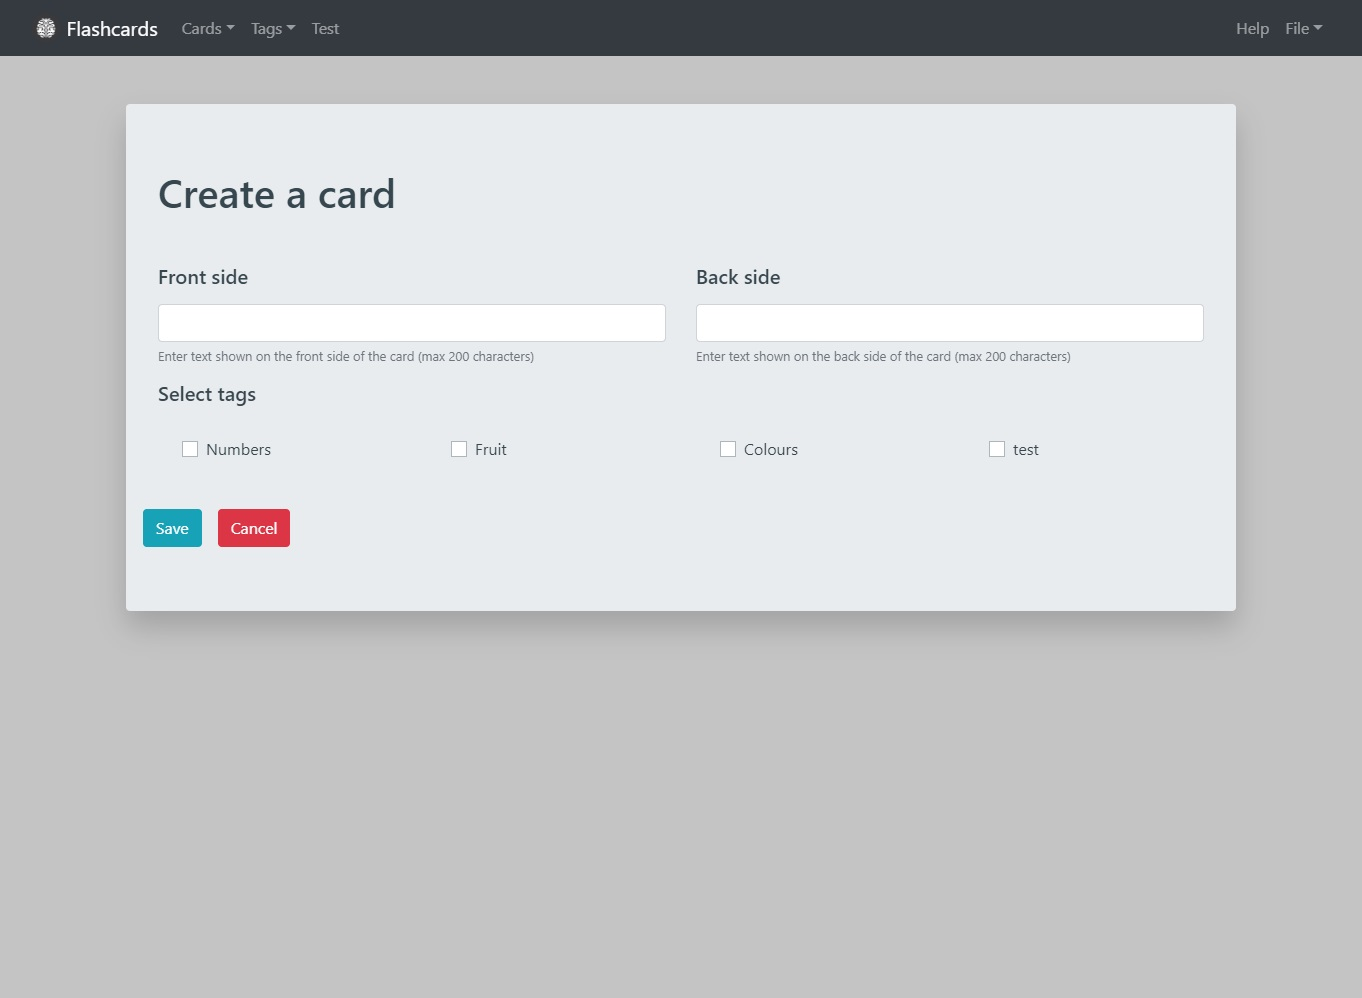
\includegraphics{assets/create_card.jpg}
\caption{Vytváření kartiček}
\end{figure}

\hypertarget{zobrazovuxe1nuxed-a-uxfaprava-kartiux10dek}{%
\section{Zobrazování a úprava
kartiček}\label{zobrazovuxe1nuxed-a-uxfaprava-kartiux10dek}}

Funkce na úpravu existujících kartiček a zobrazení všech kartiček. Pokud
budou obě upravované hodnoty změněné na již existující, aplikace
upozorní uživatele a změny se neuloží.

\begin{enumerate}
\def\labelenumi{\arabic{enumi}.}
\tightlist
\item
  Klikneme na tlačítko \textbf{Edit card} v menu liště.
\item
  Zobrazí se seznam všech existujících kartiček v tabulce.

  \begin{itemize}
  \tightlist
  \item
    Tabulka má čtyři sloupečky: text na přední straně (\textbf{Front
    side}); text na zadní straně (\textbf{Back side}); počet okruhů,
    které obsahují danou kartičku (\textbf{No.~of tags}); tlačítko na
    úpravu (\textbf{Edit}) a na smazání (\textbf{Delete}).
  \end{itemize}
\item
  Po kliknutí na tlačítko \textbf{Delete} se aplikace zeptá na potvrzení
  a poté kartičku smaže a odstraní ji ze všech okruhů.
\item
  Po kliknutí na tlačítko \textbf{Edit} se zobrazí formulář na úpravu.

  \begin{itemize}
  \tightlist
  \item
    Funguje stejně jako vytváření kartičky, s tím rozdílem, že políčka a
    zaškrtávací tlačítka jsou již předvyplněná momentálními hodnotami.
  \end{itemize}
\end{enumerate}

\begin{figure}
\centering
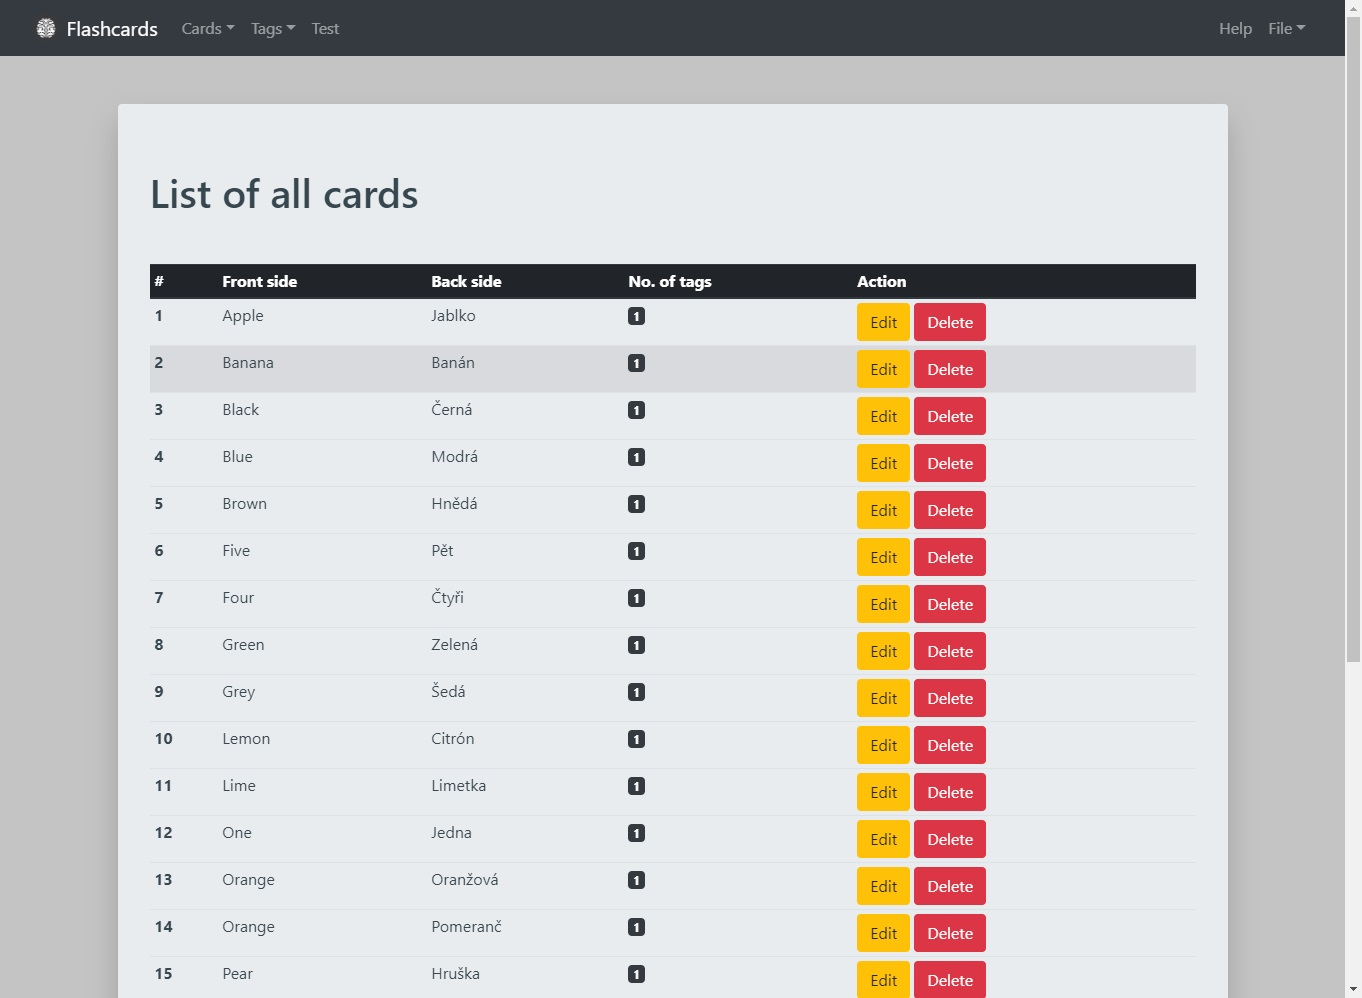
\includegraphics{assets/list_cards.jpg}
\caption{Zobrazení kartiček}
\end{figure}

\hypertarget{vytvuxe1ux159enuxed-okruhux16f}{%
\section{Vytváření okruhů}\label{vytvuxe1ux159enuxed-okruhux16f}}

Funkce na vytváření nových okruhů. Pokud okruh se zadanou hodnotou již
existuje, aplikace upozorní uživatele a nový okruh nevytvoří.

\begin{enumerate}
\def\labelenumi{\arabic{enumi}.}
\tightlist
\item
  Klikneme na tlačítko \textbf{Create tag} v menu liště.
\item
  Vyplníme políčko \textbf{Tag name} textem, který bude sloužit jako
  název nového okruhu na zkoušení (maximální délka názvu je 100 znaků).
\item
  Tlačítkem \textbf{Save} uložíme nový okruh, tlačítkem \textbf{Cancel}
  zahodíme vložený text a nový okruh se neuloží.
\end{enumerate}

\begin{figure}
\centering
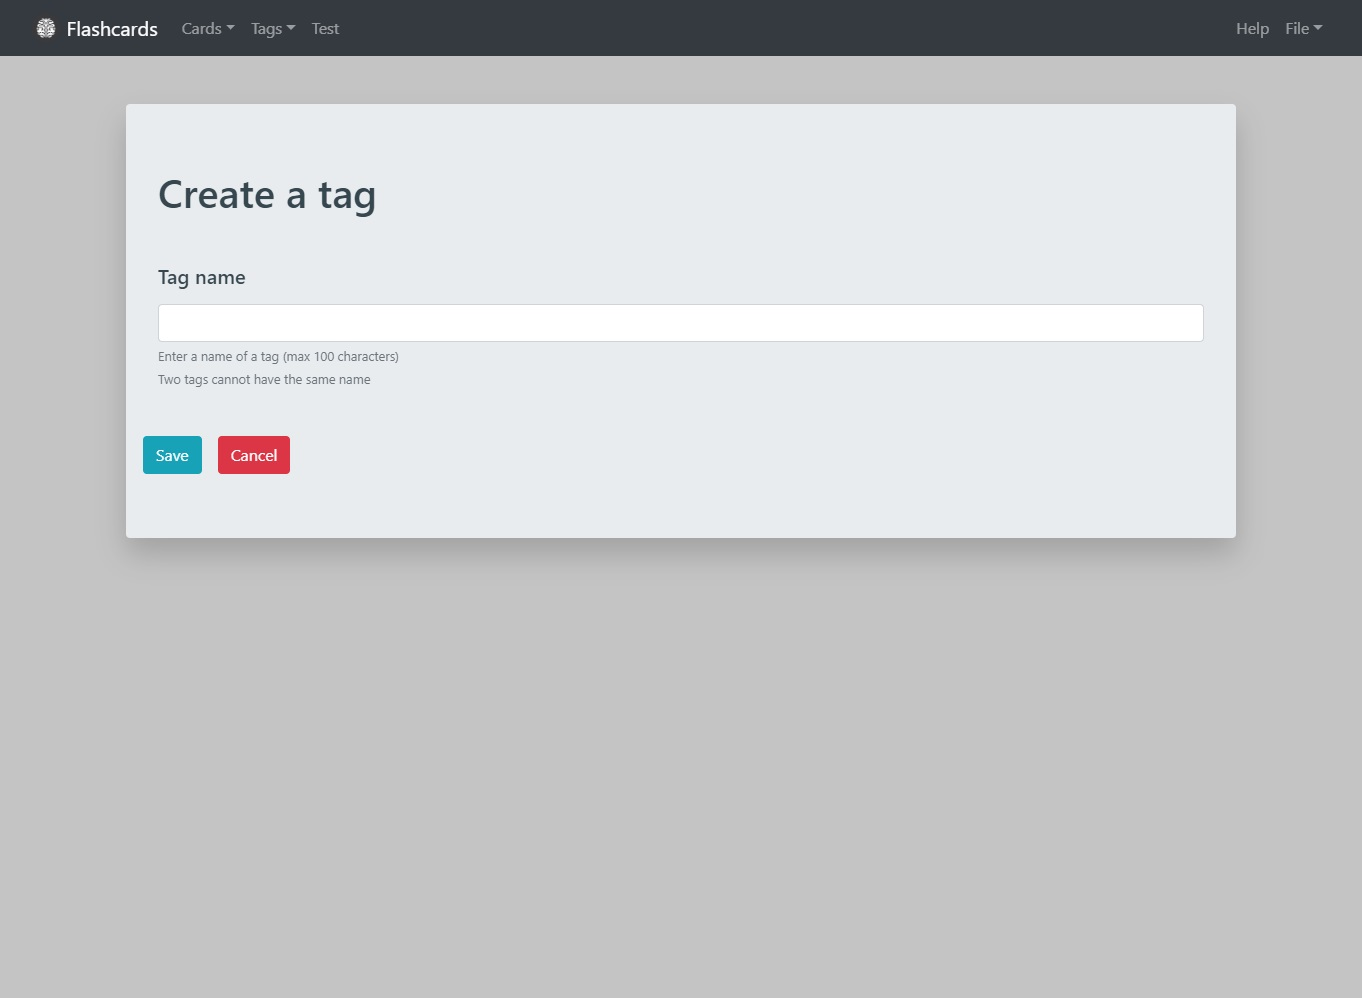
\includegraphics{assets/create_tag.jpg}
\caption{Vytváření okruhů}
\end{figure}

\hypertarget{zobrazovuxe1nuxed-a-uxfaprava-okruhux16f}{%
\section{Zobrazování a úprava
okruhů}\label{zobrazovuxe1nuxed-a-uxfaprava-okruhux16f}}

Funkce na úpravu existujících okruhů a zobrazení všech okruhů. Pokud
bude vložený text názvem již existujícího okruhu, aplikace upozorní
uživatele a změna se neuloží.

\begin{enumerate}
\def\labelenumi{\arabic{enumi}.}
\tightlist
\item
  Klikneme na tlačítko \textbf{Edit tag} v menu liště.
\item
  Zobrazí se tabulka všech existujících okruhů v tabulce.

  \begin{itemize}
  \tightlist
  \item
    Tabulka má čtyři sloupečky: název okruhu (\textbf{Name of the tag});
    počet kartiček v daném okruhu (\textbf{No.~of cards}); úspěšnost
    posledního testu daného okruhu v procentech (\textbf{Learned});
    tlačítko na úpravu (\textbf{Edit}) a na smazání (\textbf{Delete}).
  \end{itemize}
\item
  Po kliknutí na tlačítko \textbf{Delete} se aplikace zeptá na potvrzení
  a poté okruh smaže. Kartičky v okruhu zůstanou zachovány.
\item
  Po kliknutí na tlačítko \textbf{Edit} se zobrazí formulář na úpravu.

  \begin{itemize}
  \tightlist
  \item
    Funguje stejně jako vytváření okruhů, s tím rozdílem, že políčko
    \textbf{Tag name} je již předvyplněno momentální hodnotou.
  \end{itemize}
\end{enumerate}

\begin{figure}
\centering
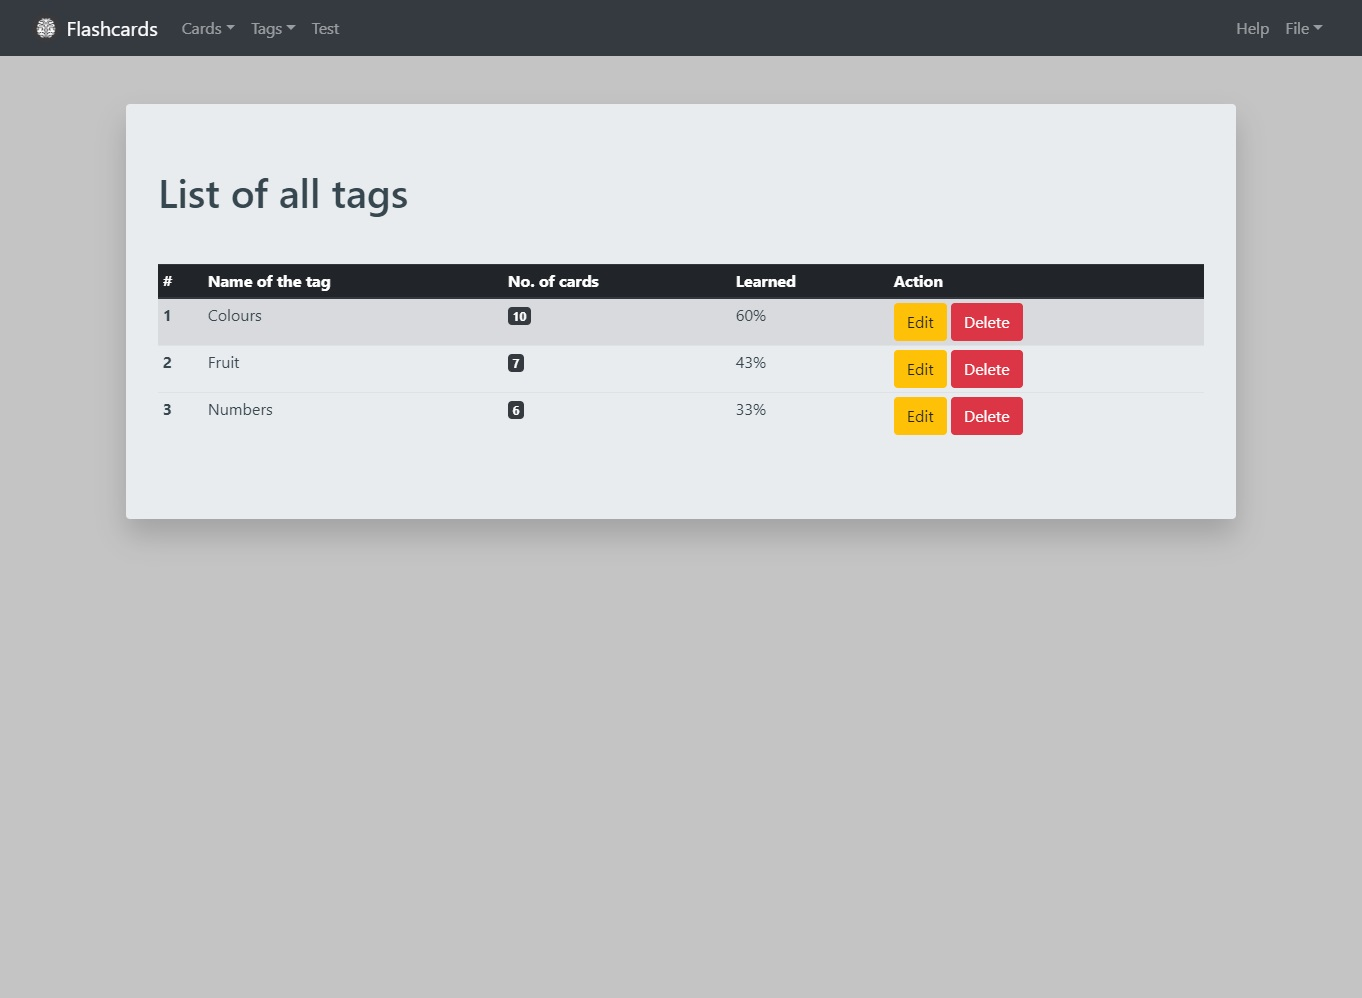
\includegraphics{assets/list_tag.jpg}
\caption{Zobrazení okruhů}
\end{figure}

\hypertarget{testy}{%
\section{Testy}\label{testy}}

Funkce spravující všechny testy. Jsou zde obsažené tři typy testů:
procházení kartiček (v aplikaci \textbf{Browse}), vybírání z možností (v
aplikaci \textbf{Choices}) a psaní správné odpovědi (v aplikaci
\textbf{Write}). V nich uživatel postupně prochází všechny kartičky
zvoleného okruhu a podle typu testu odpovídá na otázky. Při výběru
okruhu k testování si lze zvolit, kterým ,,směrem" budou kartičky
zkoušeny. Po každé odpovědi se zobrazí, zda byla odpověď správná, či
špatná. Pokud byla špatná, zobrazí se i správné řešení. V průběhu testu
je zobrazen počet zbývajících otázek a počet správných a špatných
odpovědí. Po zodpovězení všech otázek se zobrazí celková úspěšnost
testovaného okruhu, která se uloží pro budoucí porovnání, a uživatel si
může prohlédnout všechny své odpovědi.

\begin{enumerate}
\def\labelenumi{\arabic{enumi}.}
\tightlist
\item
  Klikneme na tlačítko \textbf{Test} v menu liště.
\item
  Zobrazí se seznam tlačítek, kdy každé představuje jeden okruh ke
  zkoušení.
\item
  Po kliknutí na tlačítko s názvem vybraného okruhu, který chceme
  otestovat, se zobrazí stránka na výběr typu testu.
\item
  Tlačítkem \textbf{Back to tag selection} se vrátíme na výběr okruhu.
\item
  Máme na výběr ze tří typů testů: procházení kartiček
  (\textbf{Browse}), vybírání z možností (\textbf{Choices}) a psaní
  správné odpovědi (\textbf{Write}).
\item
  Pod tlačítky je přepínač (\textbf{Reverse}), který určuje ,,směr"
  kartiček.

  \begin{itemize}
  \tightlist
  \item
    V normálním nastavení se aplikace ptá přední stranou kartičky a
    očekává odpověď zadní stranou
  \item
    Při přepnutém přepínači se aplikace bude ptát zadní stranou kartičky
    a bude očekávat odpověď přední stranou.
  \end{itemize}
\item
  Pro výběr typu testu klikneme na dané tlačítko.
\end{enumerate}

\begin{figure}
\centering
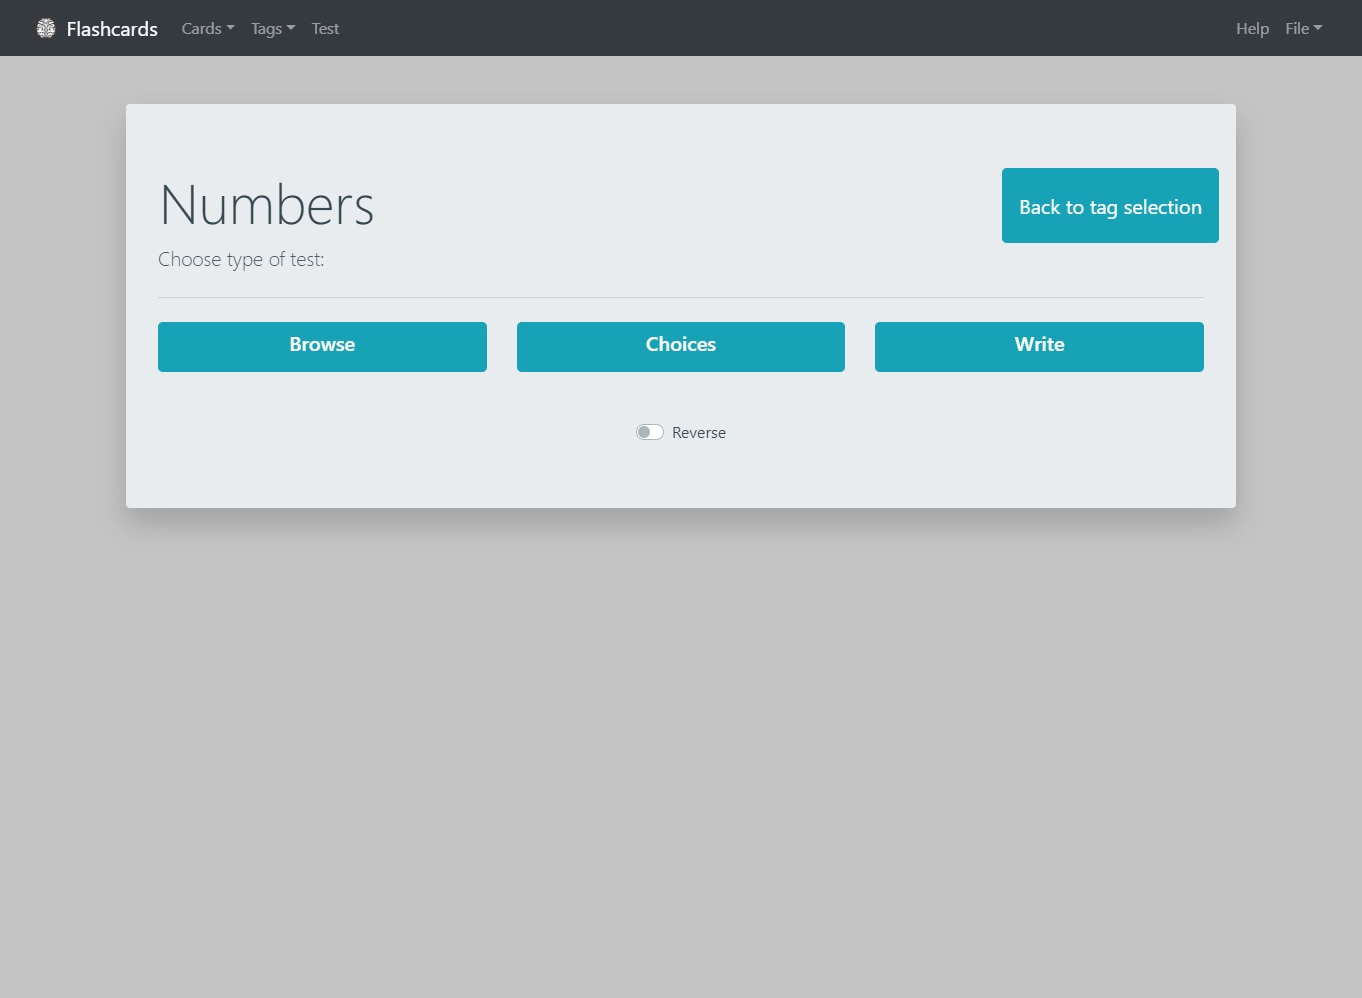
\includegraphics{assets/test_type.jpg}
\caption{Výběr typu testu}
\end{figure}

\hypertarget{test---prochuxe1zenuxed-kartiux10dek}{%
\subsection{Test - procházení
kartiček}\label{test---prochuxe1zenuxed-kartiux10dek}}

Tento test nevyžaduje žádné odpovědi, uživatel pouze postupně prochází
všechny kartičky.

\begin{itemize}
\tightlist
\item
  Kliknutím na kartičku se kartička otočí a zobrazí druhou stranu.
\item
  Kliknutím na tlačítko \textbf{Next} se zobrazí další kartička,
  tlačítko \textbf{Previous} zobrazí předchozí kartičku.
\item
  Nad kartičkami je ukazatel, který ukazuje, kolikátá kartička z
  celkového počtu je právě vidět.
\item
  Procházení ukončíme tlačítkem \textbf{Back to test selection}.
\end{itemize}

\begin{figure}
\centering
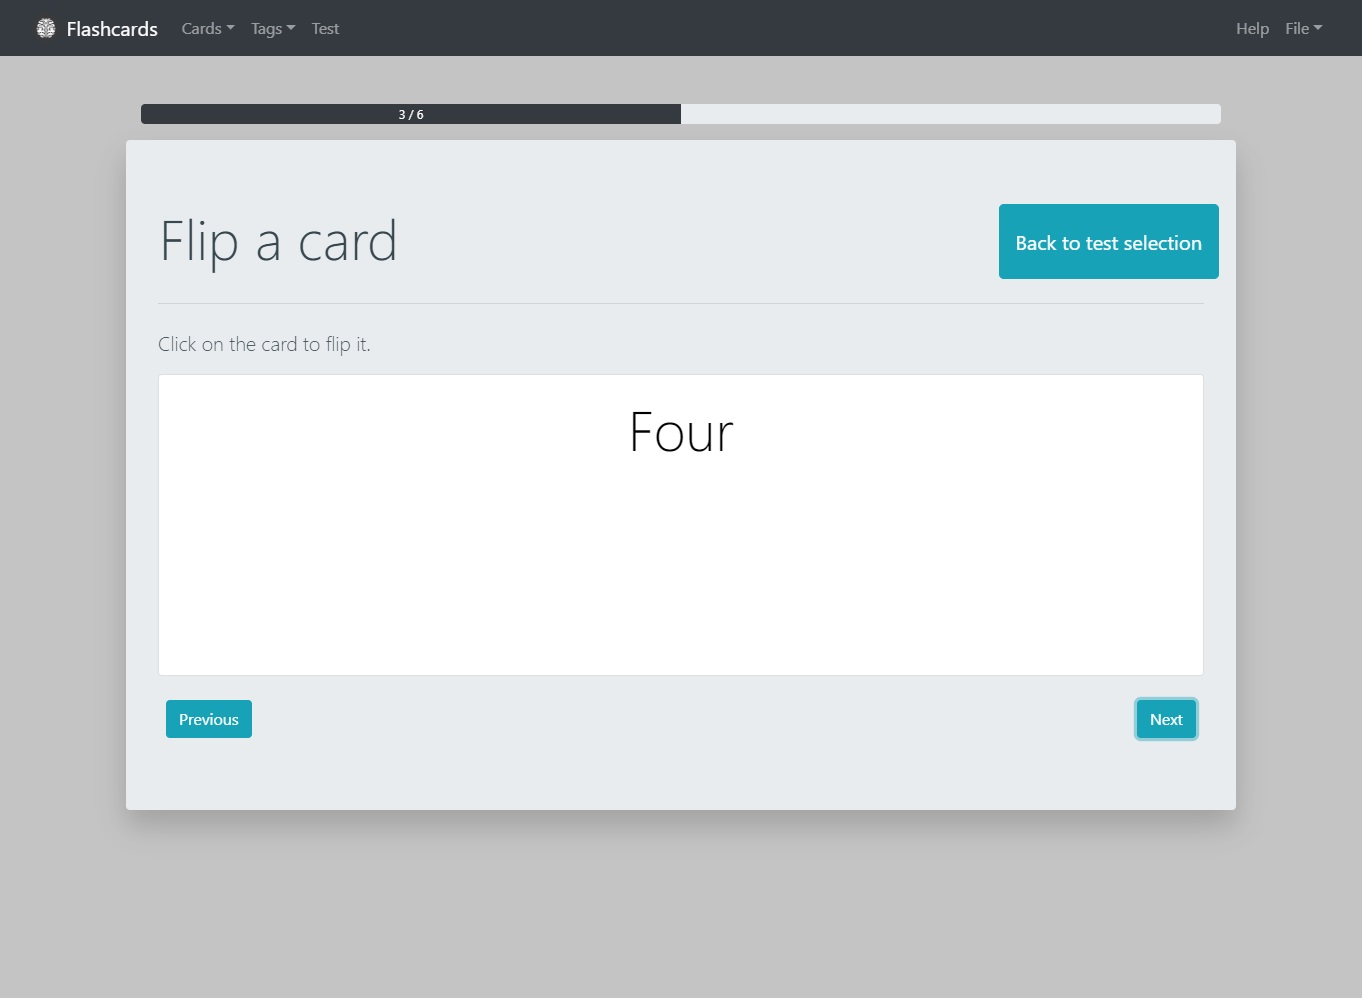
\includegraphics{assets/browse.jpg}
\caption{Procházení kartiček}
\end{figure}

\hypertarget{test---vybuxedruxe1nuxed-z-moux17enostuxed}{%
\subsection{Test - vybírání z
možností}\label{test---vybuxedruxe1nuxed-z-moux17enostuxed}}

Tento test spočívá ve vybírání správné ze čtyř možností, které aplikace
nabídne. Po každé otázce aplikace zobrazí, zda byla vybraná odpověď
správná a vybranou i správnou odpověď. Na konci testu je pak vyhodnocení
úspěšnosti testu a seznam všech odpovědí vždy se správnou možností.

\begin{itemize}
\tightlist
\item
  Nahoře je velkým nápisem napsána přední strana kartičky, pro kterou
  hledáme správnou dvojici.
\item
  Pod ní jsou možnosti, ze kterých vybíráme. Vybírá se kliknutím na
  danou odpověď.
\item
  Na pravé straně jsou tři ukazatele: počet správných odpovědí (zelená
  barva), počet špatných odpovědí (červená barva) a počet zbývajících
  otázek (černá barva).
\item
  Tlačítkem \textbf{Check answer} potvrdíme odpověď a zobrazí se
  zhodnocení.
\item
  Na stránce se zhodnocením je jediné tlačítko \textbf{Next question},
  kterým se posuneme na další otázku.
\end{itemize}

\begin{figure}
\centering
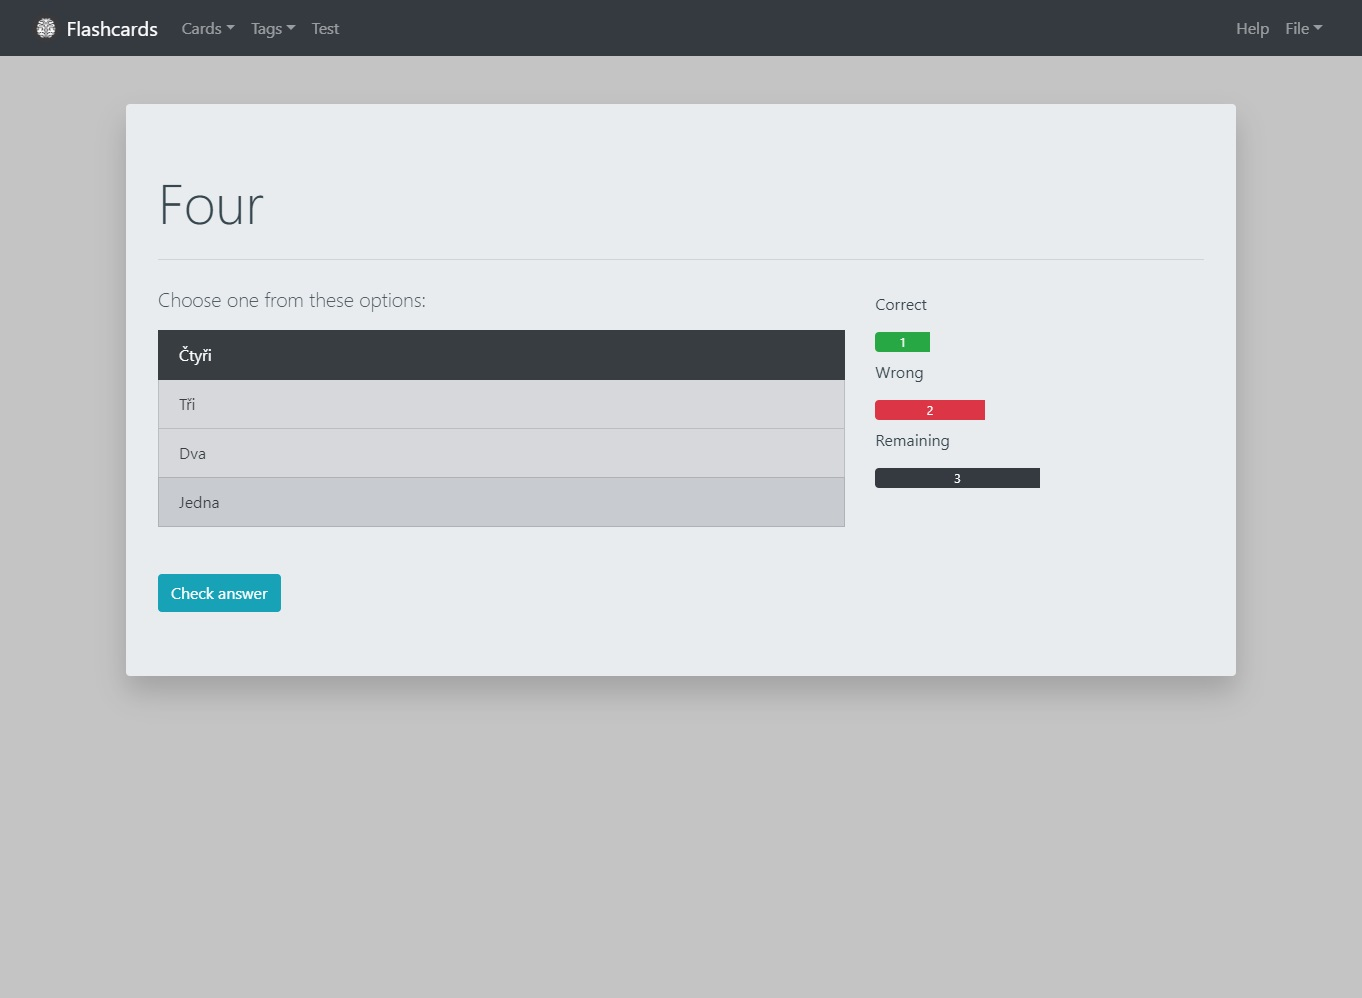
\includegraphics{assets/choices.jpg}
\caption{Vybírání z možností}
\end{figure}

Po poslední otázce se zobrazí stránka se sumarizací otázek.

\begin{itemize}
\tightlist
\item
  Je zde vypsán počet správných odpovědí, procentuální úspěšnost a
  jestli došlo ke zlepšení, nebo ke zhoršení.
\item
  Kliknutím na tlačítko \textbf{Show answers} se zobrazí seznam všech
  odpovědí.

  \begin{itemize}
  \tightlist
  \item
    Správné odpovědi jsou zvýrazněny zeleně, špatné červeně.
  \end{itemize}
\item
  Tlačítkem \textbf{Continue to test selection} se vrátíme na stránku s
  výběrem typu testu.
\end{itemize}

\begin{figure}
\centering
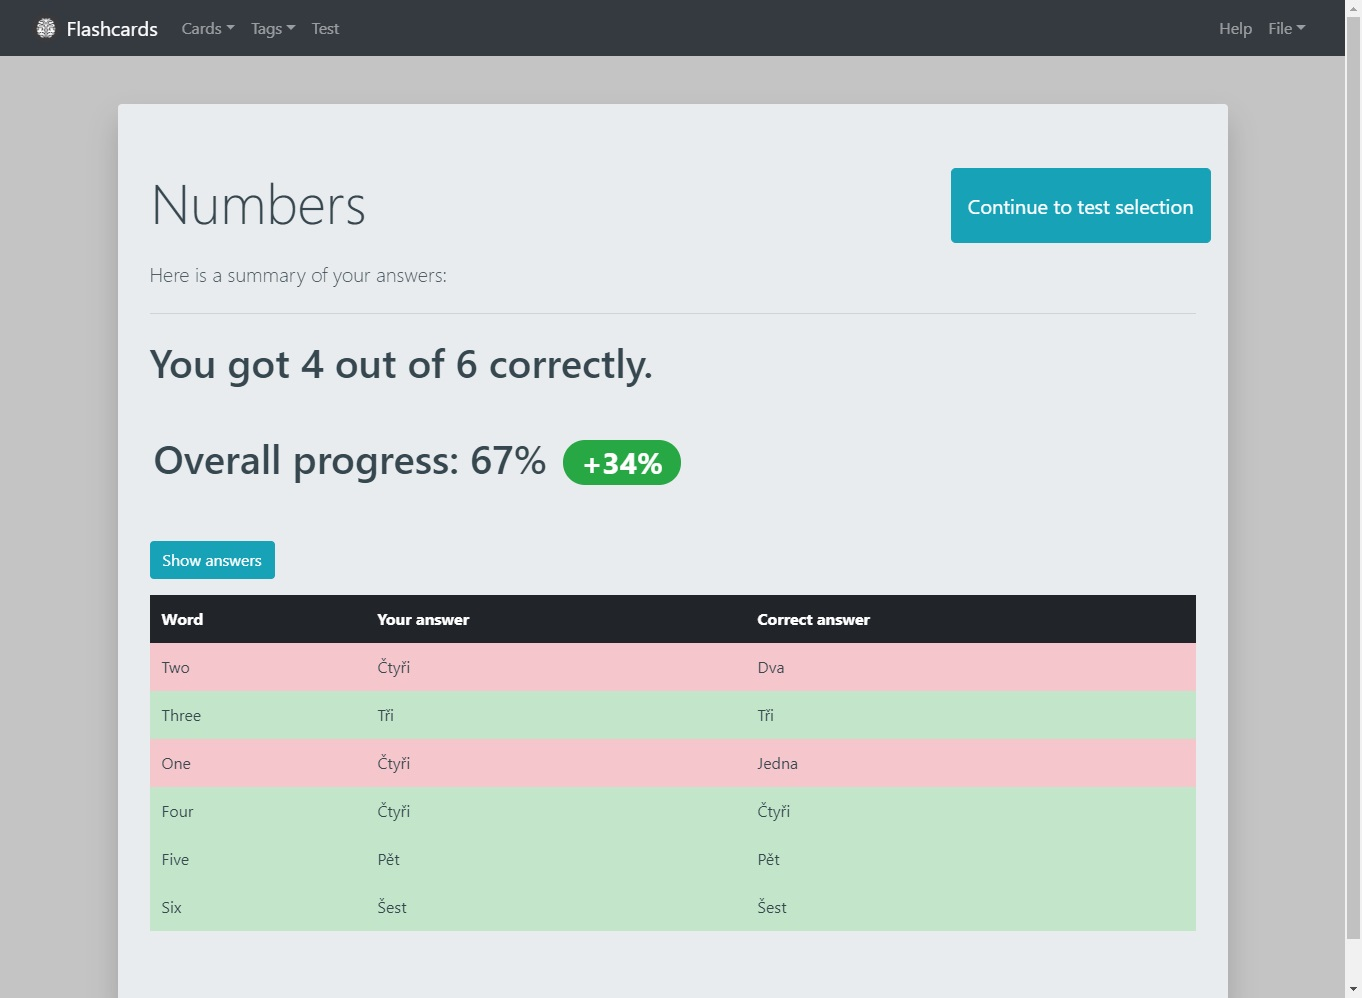
\includegraphics{assets/test_end.jpg}
\caption{Vyhodnocení testu}
\end{figure}

\hypertarget{test---psanuxed-spruxe1vnuxe9-odpovux11bdi}{%
\subsection{Test - psaní správné
odpovědi}\label{test---psanuxed-spruxe1vnuxe9-odpovux11bdi}}

Tento test spočívá v napsání správné odpovědi. Po každé otázce aplikace
zobrazí, zda byla vybraná odpověď správná a vybranou i správnou odpověď.
Aplikace toleruje překlepy podle délky slova (čím delší slovo, tím více
chyb je uznáno). Taková odpověď je vyhodnocena jako správná, ale všechny
chyby jsou zvýrazněny. Na konci testu je pak vyhodnocení úspěšnosti
testu a seznam všech odpovědí vždy se správnou možností.

\begin{itemize}
\tightlist
\item
  Nahoře je velkým nápisem napsána přední strana kartičky, pro kterou
  píšeme správnou dvojici.
\item
  Pod ní je jediné políčko, kam má být vepsána správná odpověď.
\item
  Na pravé straně jsou tři ukazatele: počet správných odpovědí (zelená
  barva), počet špatných odpovědí (červená barva) a počet zbývajících
  otázek (černá barva).
\item
  Tlačítkem \textbf{Check answer} potvrdíme odpověď a zobrazí se
  zhodnocení.
\item
  Na stránce se zhodnocením je jediné tlačítko \textbf{Next question},
  kterým se posuneme na další otázku.
\end{itemize}

\begin{figure}
\centering
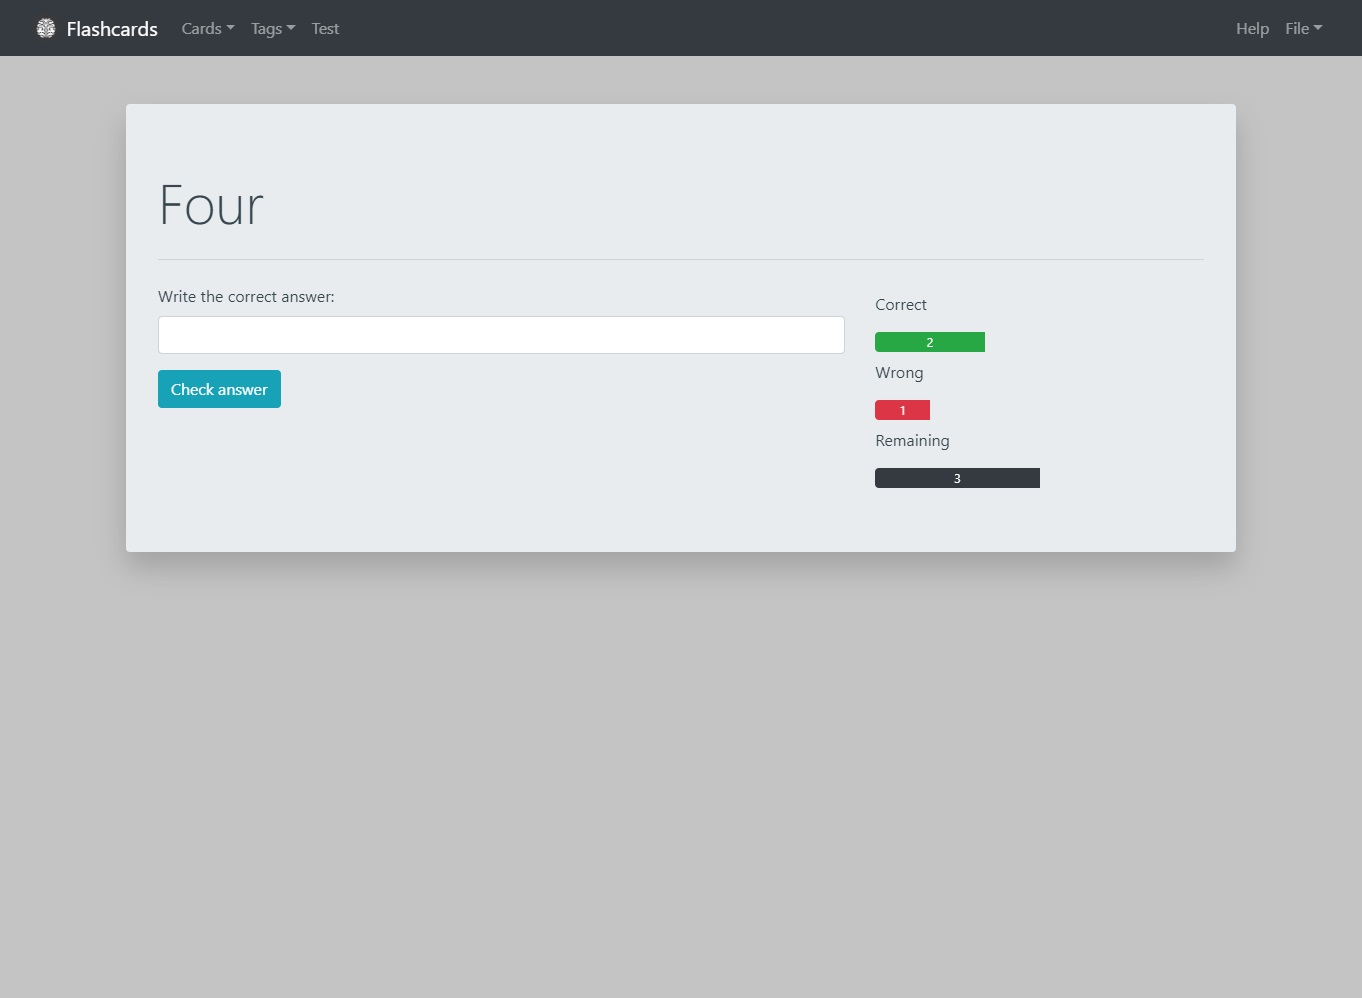
\includegraphics{assets/write.jpg}
\caption{Psaní správné odpovědi}
\end{figure}

Po poslední otázce se zobrazí stránka se sumarizací otázek.

\begin{itemize}
\tightlist
\item
  Je zde vypsán počet správných odpovědí, procentuální úspěšnost a
  jestli došlo ke zlepšení, nebo ke zhoršení.
\item
  Kliknutím na tlačítko \textbf{Show answers} se zobrazí seznam všech
  odpovědí.

  \begin{itemize}
  \tightlist
  \item
    Správné odpovědi jsou zvýrazněny zeleně, špatné červeně.
  \end{itemize}
\item
  Tlačítkem \textbf{Continue to test selection} se vrátíme na stránku s
  výběrem typu testu.
\end{itemize}

\begin{figure}
\centering
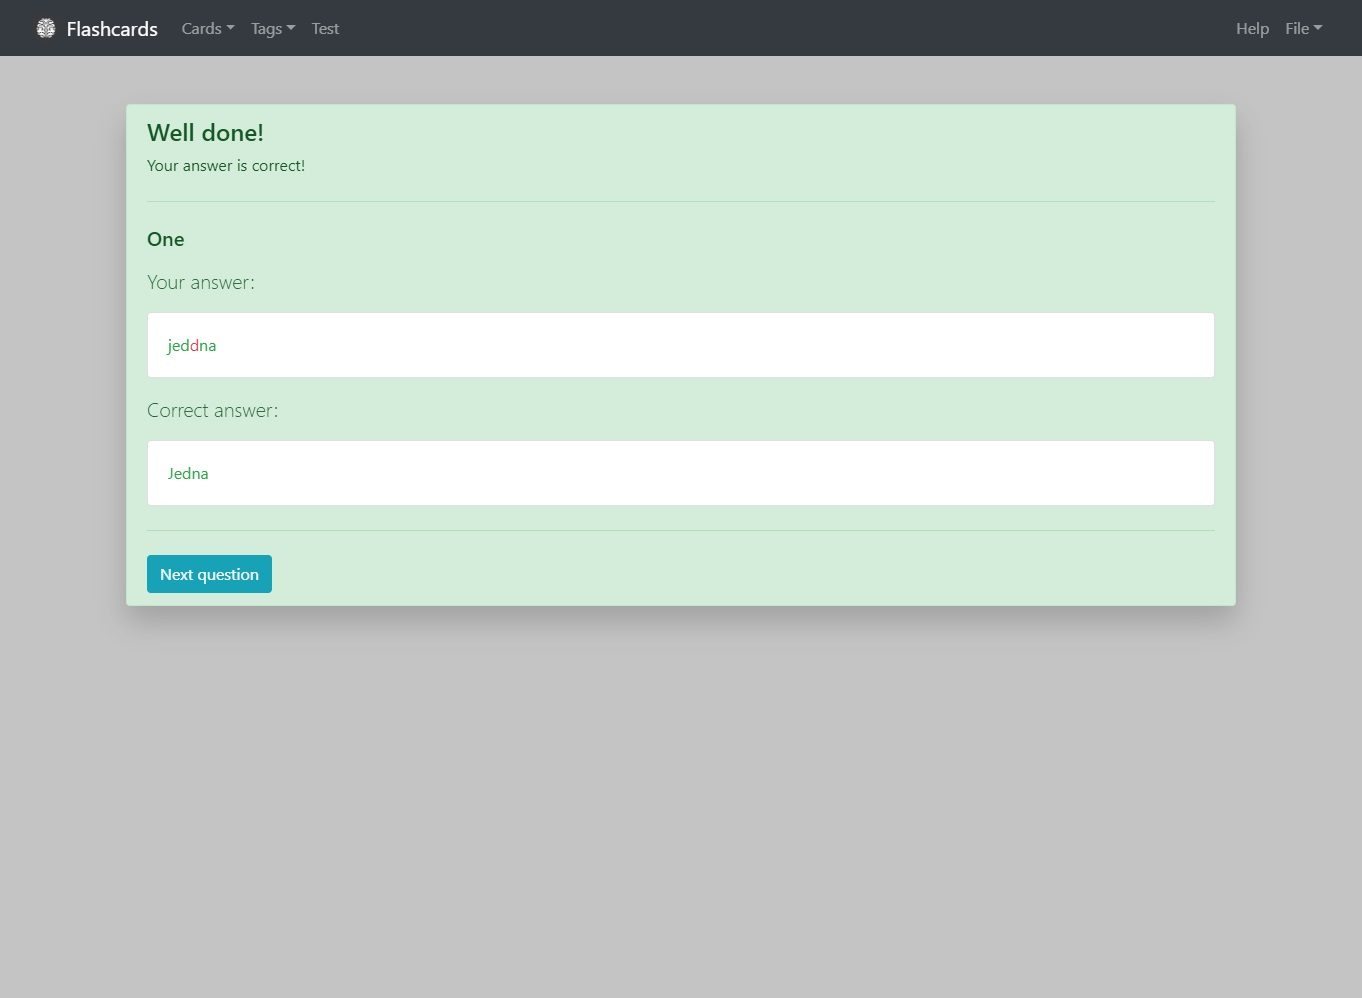
\includegraphics{assets/write_halfcorrect.jpg}
\caption{Zvýrazňování překlepů}
\end{figure}

\hypertarget{export}{%
\section{Export}\label{export}}

Funkce umožňující export všech kartiček a okruhů, které jsou právě
uložené v aplikaci. Export probíhá do \textbf{.csv} souboru, který je
uložen do složky export, ta je ve stejné složce jako spouštěcí soubor
aplikace.

\begin{enumerate}
\def\labelenumi{\arabic{enumi}.}
\tightlist
\item
  Klikneme na tlačítko \textbf{File} a pak na tlačítko \textbf{Export} v
  menu liště.
\item
  Zobrazí se stránka s jediným políčkem, kam napíšeme název
  exportovaného souboru.

  \begin{itemize}
  \tightlist
  \item
    Název může obsahovat pouze písmena a číslice.
  \item
    Název píšeme bez koncovky!
  \end{itemize}
\item
  Kliknutím na tlačítko \textbf{Confirm export} se zahájí export dat
  (může to chvíli trvat).
\item
  Po exportování se zobrazí potvrzovací okénko, že export proběhl
  správně.
\end{enumerate}

\begin{figure}
\centering
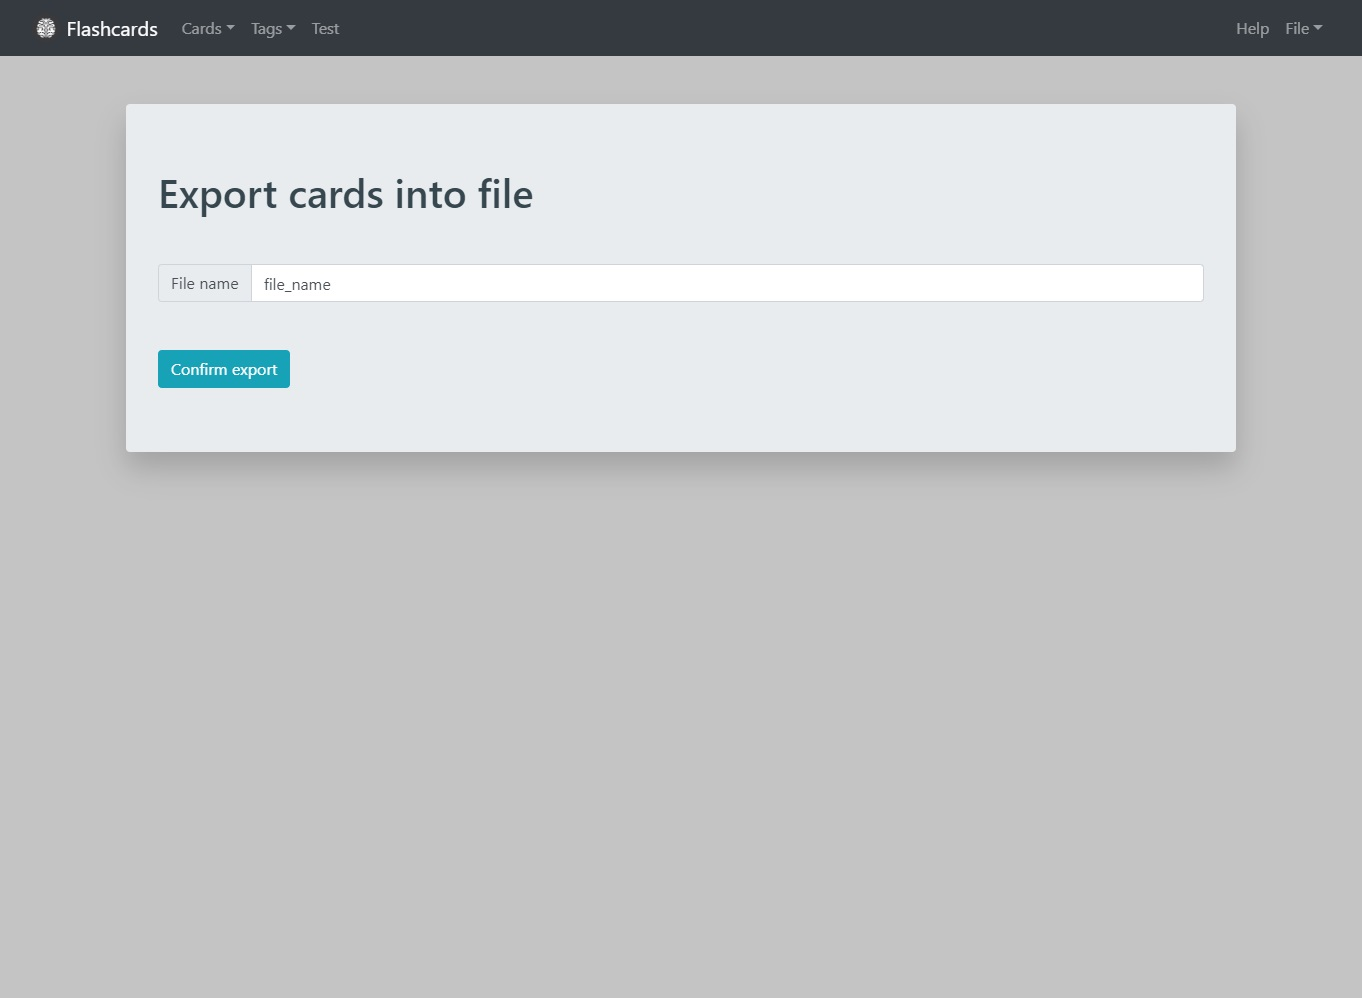
\includegraphics{assets/export.jpg}
\caption{Export}
\end{figure}

\hypertarget{import}{%
\section{Import}\label{import}}

Funkce umožňující import kartiček a okruhů ze souboru s koncovkou
\textbf{.csv}. Importovaná data musí být v přesně daném formátu (viz
níže), jinak budou přeskočena. Pokud bude mezi importovanými daty již
existující kartička, nebude se přepisovat, ani když bude v jiných
okruzích než ta momentálně uložená v aplikaci.

\begin{enumerate}
\def\labelenumi{\arabic{enumi}.}
\tightlist
\item
  Klikneme na tlačítko \textbf{File} a pak na tlačítko \textbf{Import} v
  menu liště.
\item
  Zobrazí se stránka s jediným tlačítkem, které zobrazí průzkumníka
  souborů.
\item
  V průzkumníkovi najdeme soubor, který chceme importovat.
\item
  Kliknutím na tlačítko \textbf{Confirm export} se zahájí import dat
  (může to chvíli trvat).
\item
  Po importování se zobrazí potvrzovací okénko, že byl import dokončen.
\end{enumerate}

\begin{figure}
\centering
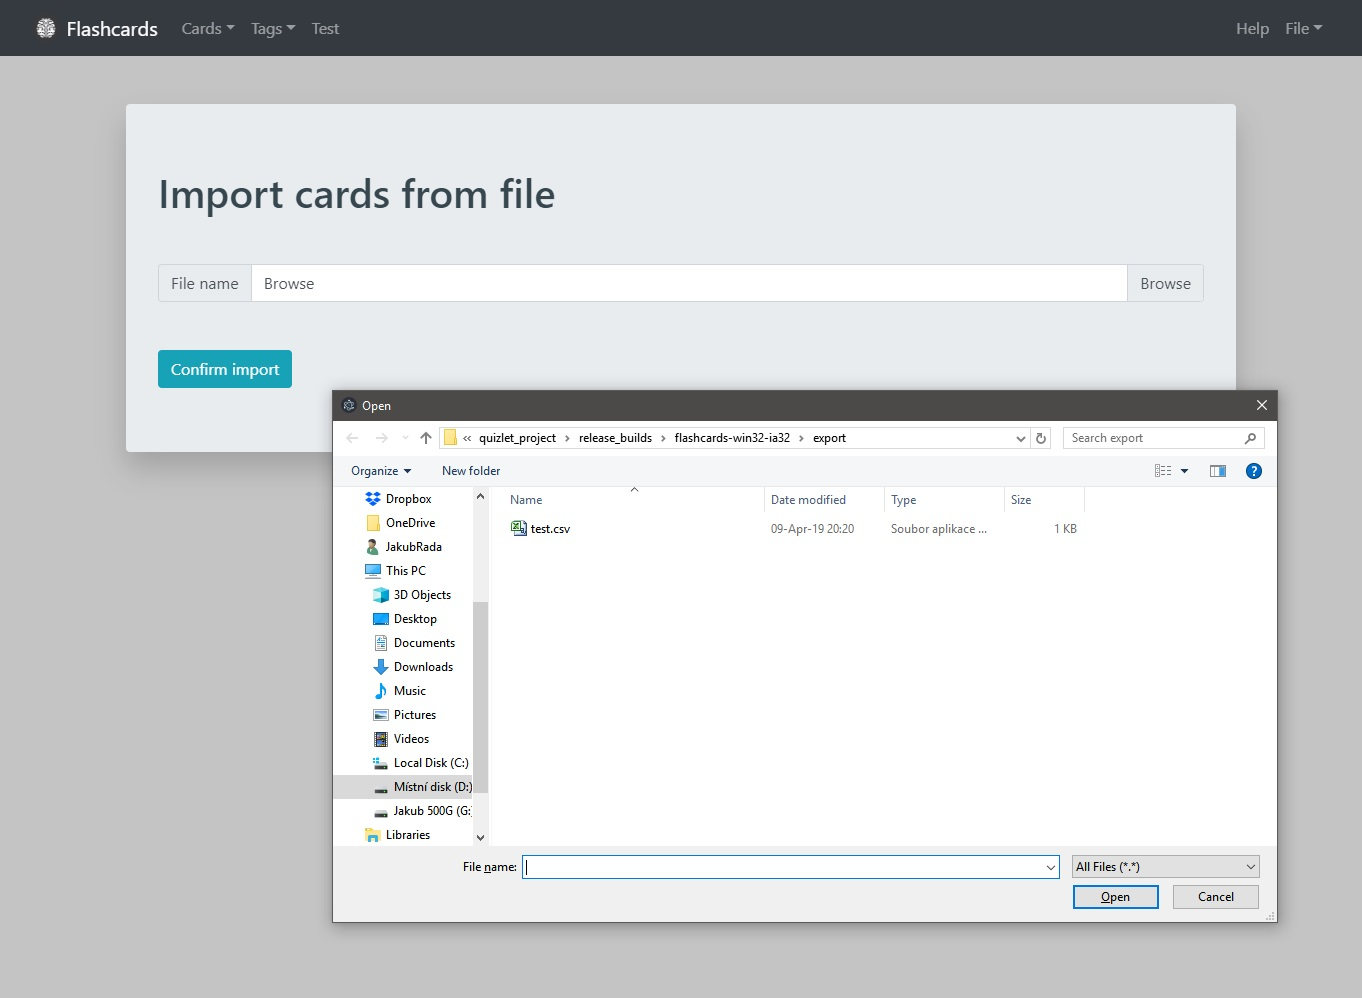
\includegraphics{assets/import.jpg}
\caption{Import kartiček ze souboru}
\end{figure}

Formát \textbf{.csv} souboru

\begin{itemize}
\tightlist
\item
  Okruh

  \begin{itemize}
  \tightlist
  \item
    tag, číslo okruhu (počítají se jenom ty v tomto souboru), název
    okruhu
  \item
    například: \texttt{tag,\ 1,\ Čísla}
  \end{itemize}
\item
  Kartička

  \begin{itemize}
  \tightlist
  \item
    card, přední strana kartičky, zadní strana kartičky, čísla okruhů,
    do kterých kartička patří, oddělené ,,\textbar{}" (čísla okruhů v
    tomto souboru)
  \item
    například: \texttt{card,\ One,\ Jedna,\ 1\textbar{}2\textbar{}3}
  \end{itemize}
\item
  Každý záznam píšeme na samostatný řádek
\end{itemize}

Ukázkový soubor s daty k importu

\begin{verbatim}
    tag, 1, Numbers
    tag, 2, Fruit
    tag, 3, Colours
    card, Five, Pět, 1
    card, Banana, Banán, 2
    card, Four, Čtyři, 1
    card, Apple, Jablko, 2
    card, White, Bílá, 3
    card, Blue, Modrá, 3
\end{verbatim}

\hypertarget{nuxe1povux11bda}{%
\section{Nápověda}\label{nuxe1povux11bda}}

Kliknutím na tlačítko \textbf{Help} v menu liště se zobrazí rychlá
nápověda v angličtině.
\clearpage
\hypertarget{zdroje}{%
\section{Zdroje}\label{zdroje}}

\hypertarget{pouux17eituxe9-knihovny}{%
\subsection{Použité knihovny}\label{pouux17eituxe9-knihovny}}

\begin{itemize}
\tightlist
\item
  \textbf{npm 6.4.1} \href{https://www.npmjs.com/}{www.npmjs.com}
\item
  \textbf{Electron 4.1}
  \href{https://electronjs.org/}{www.electronjs.org}
\item
  \textbf{Electron packager}
  \href{https://github.com/electron-userland/electron-packager}{www.github.com/electron-userland/electron-packager}
\item
  \textbf{Bootstrap 4.2}
  \href{https://getbootstrap.com/}{www.getbootstrap.com}
\item
  \textbf{JQuery 3.3} \href{https://jquery.com/}{www.jquery.com}
\item
  \textbf{Python 3.7} \href{https://www.python.org/}{www.python.org}
\item
  \textbf{Django 2.1.5}
  \href{https://www.djangoproject.com/}{www.djangoproject.com}
\item
  \textbf{LaTeX}
  \href{https://www.latex-project.org/}{www.latex-project.org}
\item
  \textbf{JavaScript}
  \href{https://www.javascript.com}{www.javascript.com}
\end{itemize}

\hypertarget{dokumentace}{%
\subsection{Dokumentace}\label{dokumentace}}

\begin{itemize}
\tightlist
\item
  \textbf{Electron docs}
  \href{https://electronjs.org/docs}{www.electronjs.org/docs}
\item
  \textbf{Django docs}
  \href{https://docs.djangoproject.com/en/2.1/}{www.docs.djangoproject.com/en/2.1}
\item
  \textbf{DevDocs} \href{https://devdocs.io/}{www.devdocs.io}
\item
  \textbf{Electron packager tutorial}
  \href{https://www.christianengvall.se/electron-packager-tutorial/}{www.christianengvall.se/electron-packager-tutorial}
\item
  \textbf{Bootstrap docs}
  \href{https://getbootstrap.com/docs/4.2/getting-started/introduction/}{www.getbootstrap.com/docs/4.2}
\item
  \textbf{JQuery API} \href{https://api.jquery.com/}{www.api.jquery.com}
\item
  \textbf{W3Schools}
  \href{https://www.w3schools.com/html/default.asp}{www.w3schools.com/html/default.asp}
\item
  \textbf{Pandoc} \href{https://pandoc.org/}{www.pandoc.org}
\item
  \textbf{StackOverflow}
  \href{https://stackoverflow.com/}{www.stackoverflow.com}
\end{itemize}

\hypertarget{ikony-a-obruxe1zky}{%
\subsection{Ikony a obrázky}\label{ikony-a-obruxe1zky}}

\begin{itemize}
\tightlist
\item
  \textbf{IconFinder}
  \href{https://www.iconfinder.com/search/?q=brain\&price=free}{www.iconfinder.com/search/?q=brain\&price=free}
\item
  \textbf{Obrázek na titulní straně}
  \href{http://www.inspiregroup.co.nz/whats-happening/category/brain-science/}{www.inspiregroup.co.nz/whats-happening/category/brain-science}
\end{itemize}
\end{document}